\section{Kasutajaliidese disain}
\label{chapters:analysis_interface_design}
MVP funktsionaalsusega (osa \ref{chapters:analysis_requirements}) prototüübi  realiseerimiseks on vaja luua
veebirakenduse kasutajaliidesele järgmised vaated:
\begin{itemize}
    \item Menüüriba
    \item Registreerimise ja sise logimise vaated
    \item Dashboard-vaate
    \item Kasutaja andmete vaade
    \item Ehitusmaterjalide nimekirja vaade
    \item Ehitusmaterjali loomise ja redigeerimise vaade
    \item Kalkulaatori vaade
    \item Kasutajate nimekiri (administraator)
    \item Parameetrite ja lisaandmete vaade (administraator)
\end{itemize}

Mõned vaated on rollispetsiifilised (nt kasutajate nimekirja administraatori vaade), teised on universaalsed - 
kasutajarolli alusel kasutajaliideses otsustatakse, kas näidata (või lubada) midagi kasutajale või mitte.
Igal tegevusel kontrollitakse kasutajaõigusi täiendavalt ka serveriosas enne tegevuse algust.

Kasutajaliidese disaini projekteerimine on teostatud veebipõhise tarkvaraga \textbf{Figma}. Figma võimaldab 
mugaval viisil luua ja redigeerida lehtede visuaalsed prototüübid ja seostada erinevad vaated omavahel. 

Arendatava veebirakenduse kasutajaliidese disain on minimalistlik, aga samas kaasaaegne. Kasutatakse värvilisi ikoone ja värve
elementide kujunduses, et vältida ülemääraselt ametliku mulje tekkimist. Värvitoonid on valitud selliselt, et 
välimus oleks lakooniline ja professionaalne.

Pealehel (\textit{Dasboard}) näidatakse kaardid, mille kaudu kasutajat juhitakse tööriistadele ja 
moodulitele, millele on kasutajal ligipääs. Administraatori ja tavakasutaja \textit{Dashboard}-vaated
on vastavalt erinevad. \textit{Dashboard}-kaartide näide on toodud pildil \ref{fig:desing_dashboard_cards}.
\begin{figure}[ht]
    \centering
    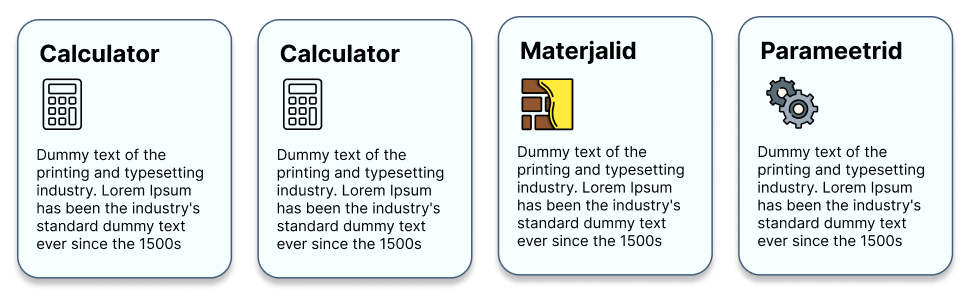
\includegraphics[width=1\textwidth]{figures/analysis/desing_dashboard_cards.png}
    \caption[Pealehe kaartide disaini näide]{\textit{Pealehe kaartide disaini näide}}
    \label{fig:desing_dashboard_cards}
\end{figure}


Kasutajaliideses kasutatakse kaks põhilist nuppude stiili - aktsepteerimise ja tühistamise nupud.
\begin{figure}[ht]
    \centering
    
\includegraphics[width=0.4\textwidth]{figures/analysis/desing_buttons.png}
    \caption[Nuppude disaini näide]{\textit{Nuppude disaini näide}}
    \label{fig:design_buttons}
\end{figure}




